\section{Experiments}\label{sec:experiments}
We compute the constants of Sections~\ref{sec:general}--\ref{sec:population} exactly for trained models with the solver of Section~\ref{sec:population}. Every population $P$ is a held-out or target empirical law mixed with a uniform mass of $1\%$ over profiles and labels, which gives full support; every design is pointwise unbiased; and every reported constant is certified by primal and dual bounds that agree to a relative error of at most $10^{-4}$. We report $W_{\rm fixed}/W_r$, the factor by which the best design of a class needs more records than the best branching design. Oracle designs are optimized at $P$; fitted designs are optimized on separate reference records and evaluated at $P$. Protocols, sample sizes, per-task values and sensitivity analyses are in Appendix~\ref{app:F}.

\paragraph{Forest updates across caps.}
On WDBC, Spambase and Ionosphere \citep{wolberg1993,spambase1999,ionosphere1989}, an old and a new random forest of twenty depth-$b$ trees are trained on disjoint records with $m\in\{6,9,12\}$ median-binarized features, and the remaining 269, 3,101 and 171 records define $P$. Table~\ref{tab:capgrid} reports the exact ratio for caps 2, 3 and 4. At cap three the best pre-committed design needs a median 1.51 times as many records as the best branching design (maximum 1.85), and the ratio grows from 1.38 at $m=6$ to 1.64 at $m=12$. The medians at caps 2 and 4 are 1.31 and 1.24. Designs fitted on training records realize ratios within a median 3\% of the exact ones on the same tasks at every cap. Branching restricted to the forests\textquotesingle{} own trees captures a median of only 17\% of the log-gain at cap three: the optimal branching designs mix many trees that neither forest contains.

\begin{table}[t]
\centering
\caption{Exact records ratio $W_{\rm fixed}/W_{\rm branch}$ for independently retrained forest updates of depth $b$ with cap $b$ on WDBC, Spambase and Ionosphere: median [10th, 90th percentile] over binding tasks, medians by number of candidate features $m$, median ratio realized by designs fitted on training records, and median share of the log-gain captured when branching may use only the forests\textquotesingle{} own trees; -- marks cells not computed.}
\label{tab:capgrid}
\footnotesize
\setlength{\tabcolsep}{2.4pt}
\begin{tabular}{rrlrrrrr}
\toprule
$b$ & tasks & median [p10, p90] & $m{=}6$ & $m{=}9$ & $m{=}12$ & fitted & own \\
\midrule
2 & 45 & 1.31 [1.21, 1.44] & 1.31 & 1.25 & 1.34 & 1.31 & 49\% \\
3 & 180 & 1.51 [1.33, 1.74] & 1.38 & 1.52 & 1.64 & 1.67 & 17\% \\
4 & 15 & 1.24 [1.15, 1.31] & 1.24 & -- & -- & 1.27 & 26\% \\
\bottomrule
\end{tabular}
\end{table}


\paragraph{Screening questionnaires.}
A depth-$b$ screening tree asks at most $b$ questions per person, so a validation study under the same burden must respect the cap. We train class-balanced CART trees on twelve yes/no items of the CDC Diabetes Health Indicators, derived from the Behavioral Risk Factor Surveillance System (BRFSS; 253,680 respondents, target diabetes or prediabetes) \citep{cdcdiabetes2017}, and on twelve binarized thyroid items (7,200 patients, abnormal function) \citep{quinlan1986thyroid}, and validate them on a disjoint random half or on respondents of the other sex. Branching asks the tree's own questions and attains the full-information variance. Table~\ref{tab:screening} shows that the gain depends on how many questions the screening decision needs. On BRFSS the best pre-committed design needs a median of 1.35--1.58 times as many respondents at caps 4 to 6. One more round removes most of this cost: at caps 4, 5 and 6 (at $b=6$ for 1 of the six trees) the exact optimal two-round design needs a median 1.00 times as many, recovering a median 100\% of the log-gap and at least 90\% in each of the 13 runs with a gain, against 33\%--63\% for following the root question and then a fixed form. Over the 21 runs with a gain, the optimized path-set design of Proposition~\ref{prop:uppermain} is within a median 2.0\% (at most 3.9\%) of the best fixed design, so the bracket between the lower end and this upper end is narrow and computable from reference data, whereas the completion-only end $N_P$ overstates the loss by a median factor 4.3. On thyroid every tree, up to depth six, depends on at most $b$ items, so $\Gamma_P=1$ and pre-commitment costs nothing intrinsic; the lower end detects this from reference data, and the rule \emph{reference lower end at most 1.05 $\Rightarrow$ no material gain} has no misses over all screening runs and forest tasks (Appendix~\ref{app:capsens}). 

\begin{table}[t]
\centering
\caption{Screening trees: records needed relative to branching, which asks the tree\textquotesingle s own questions (medians over targets and seeds). Best, Fitted: optimal fixed design at the target law and on source records. Two: exact optimal two-round design (at $b=6$ for 1 of six trees; not computed for 21 items, --); H2: following the root question, then the best fixed form. Lower, PS, $N_P$: the lower end of Theorem~\ref{thm:bracket}, the optimized path-set end of Proposition~\ref{prop:uppermain} and the completion-only end.}
\label{tab:screening}
\footnotesize
\setlength{\tabcolsep}{2.4pt}
\begin{tabular}{lrrrrrrr}
\toprule
Data, $b$ & Best & Fitted & Two & H2 & Lower & PS & $N_P$ \\
\midrule
BRFSS, 4 & 1.49 & 1.57 & 1.00 & 1.14 & 1.18 & 1.53 & 3.6 \\
BRFSS, 5 & 1.35 & 1.42 & 1.00 & 1.21 & 1.08 & 1.36 & 5.9 \\
BRFSS, 6 & 1.58 & 1.68 & 1.00 & 1.39 & 1.13 & 1.61 & 11.4 \\
Thyroid, 3--6 & 1.00 & 1.04 & 1.00 & -- & 1.00 & 1.00 & 5.0 \\
\addlinespace[2pt]
BRFSS-21, 3 & 1.00 & 1.00 & 1.00 & -- & 1.00 & 1.00 & 1.5 \\
BRFSS-21, 4 & 1.46 & 1.54 & -- & -- & 1.17 & 1.50 & 3.8 \\
\bottomrule
\end{tabular}
\end{table}


\begin{figure}[t]
\centering
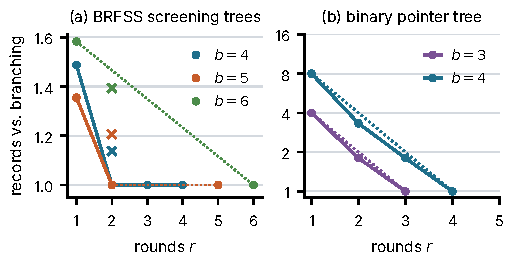
\includegraphics[width=\columnwidth]{figures/v14_rounds.pdf}
\caption{Records needed relative to branching as a function of the number of rounds ($r=1$: fixed forms; $r=b$: branching). (a) BRFSS screening trees, exact optimal $r$-round designs (median over targets and seeds); crosses mark the heuristic second round of following the root question; dotted segments join round counts that were not computed. (b) Binary pointer tree under the uniform law, a lower bound on $V_r$ (Appendix~\ref{app:pointerexact}); dotted lines are the upper bounds $2^{b-r}$ of Theorem~\ref{thm:rounds}(a).}
\label{fig:rounds}
\end{figure}

\paragraph{All 21 survey variables.}
With all 21 BRFSS variables the profile cube has $2^{21}$ elements and the form program has 1,330 forms at $b=3$ and 5,985 forms at $b=4$; the solver certifies the optimal fixed design without enumerating the cube, in a median of 6 minutes at $b=4$ on one core. At $b=3$ every tree depends on at most $b$ items, so $\Gamma_P=1$ and there is no gain. At $b=4$ the best pre-committed design needs a median 1.46 times as many respondents (maximum 1.55), the fitted design 1.54, and the optimized path-set end lies at 1.50 (Table~\ref{tab:screening}, Appendix~\ref{app:scale}).

\paragraph{Information versus design.}
Imputation from complete source records uses information that the capped audit does not collect, and it is only as good as the transport of the conditional law of unasked items. When that law transports, as under the random-half and sex splits, regression imputation and multiple imputation attain RMSE 0.89--0.99 times that of branching with coverage 0.940--0.993, and they are the better tool. Under the education shift at both caps and the poor-health shift at $b=5$, regression imputation is biased by up to 1.73 branching standard deviations and covers 0.515--0.902 of the time, multiple imputation covers 0.667--0.935, and branching and the fitted fixed form stay unbiased with coverage 0.940--0.960. Under the cost-barrier shift at both caps and the poor-health shift at $b=4$ imputation stays close to nominal (bias at most 0.23 standard deviations). The design-based scores need neither the reference nor the transport assumption, and that is the setting in which within-record adaptivity matters (Table~\ref{tab:shift}).

\paragraph{Order effects.}
If the last of $b$ answers flips with probability $0.1$ and earlier ones proportionally less often, both designs are biased: on BRFSS the median absolute bias at $n=1000$ is 1.54 clean branching standard errors for branching and 2.17 for the fitted fixed form, comparable to the sampling gains above, and branching keeps the smaller RMSE in 24 of 24 runs (Appendix~\ref{app:measurement}).

\paragraph{A real planned-missing archive.}
PISA 2012 assigned three questionnaire forms at random, and no U.S. student answered all nine predictors of our block-averaged forest ensembles; every block pair appears on a form, so a Brier contrast is identifiable from the actual menu, and optimized form scores, a block-pair Horvitz--Thompson score and multiple imputation agree (Appendix~\ref{app:pisa}). The archive demonstrates identification from real fixed forms and has no branching counterfactual.
